\chapter{Conceitos Gerais de IoT}
\label{chapter:coneceitos}

No capítulo \ref{chapter:intro}, foram vistos as bases para se implementar um projeto de IoT. A área começou a receber fortes investimentos e atenção por volta de 2009 \cite{Rampim:iot} e desde então foram feitas consideráveis implementações utilizando tecnologias e protocolos diferentes. Neste capítulo serão apresentados algumas dessas variantes, para fins de comparação e respaldo para importância e objetivo deste projeto.

\section{As Camadas da IoT}
\label{section:camadas_iot}

Uma rede IoT pode ser divida em camadas que exercem funções específicas no transporte de dados, de uma forma semelhante a redes de computadores, a camada acima não precisa saber como a inferior funciona, formando uma estrutura de pilha como na \ref{fig:1.2.0/camadas_iot}.

\begin{figure}[h!]
\centering
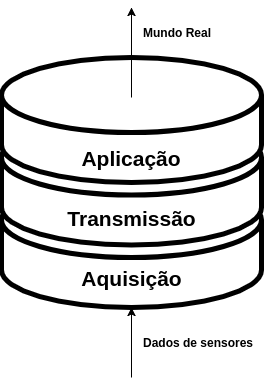
\includegraphics[width=5cm]{./02_Capitulos/02_Cap1/figures/iot_stack}
\caption{As três camadas do IoT, dos sensores ao mundo real}
\label{fig:1.2.0/camadas_iot}
\end{figure}

A primeira camada é a de aquisição de dados, que lida com o mundo físico e captura estes dados através de sensores e conversores A/D, também realiza o processamento para entregar em um formato adequado para transmissão e inteligível para aplicações que recebem os dados. A etapa de aquisição está inserida diretamente no contexto de dados físicos, geralmente são hardwares menos complexos, focados em processamento de dados e entrada e saída com conversão analógico-digital. Se comunicam com sensores ou centrais de controle lógico.

A segunda camada é a camada de transmissão, na qual estão, efetivamente, as camadas de rede embutidas. Como o nome já denuncia, ela lida com os aspectos de rede e comunicação para que o dados cheguem seus destinos. Esta camada é o coração do IoT. Na transmissão define quais dispositivos eletrônicos e suas especificação técnicas. Também define como os softwares da camada de aplicação e aquisição devem ser implementados baseado na estrutura da pilha de rede.

 E por último temos a camada de aplicação, a mais abrangente e que envolve maior poder computacional. Ela recebe os dados e lida com os processos de aplicação destes dados, seja análise, visualização, armazenamento ou a estruturação dos mesmos. A camada de aplicação encabeça a pilha do IoT. É ela que de fato trata os dados. Ela disponibiliza os dados para o mundo real, podendo exercer múltiplas funções simultâneas incluindo:

\begin{itemize}
\item Armazenamento e Análise, através de Bancos de Dados e Serviços;
\item Visualização; Aplicações Web, disponibilizando gráficos e tabelas de dados;
\item Inteligência e aprendizado, com Machine Learning e Estatística para decisões e classificação;
\item Serviços e servidores . Aplicações em nuvem fornecendo micro-serviços em aplicações Web;
\end{itemize}


\section{Tecnologias em IoT}
\label{section:tecnologias_iot}

As primeiras aplicações de IoT foram realizadas em laboratórios através de RFID \cite{Rampim:iot}, junto com códigos bidimensionais (como o QR Code), para aplicações de identificação de objetos.  É uma das soluções mais populares e de baixo custo de IoT utilizando Radio frequência.

Redes que utilizam bandas restritas (NB-IoT) visando baixo consumo e curta distância de transmissão, são utiizadas em redes IoT de celulares e irão se tornar opções dominantes de conectivdade com o advento do 5G. As NB-IoT concentram-se especificamente na cobertura, baixo custo, longa duração da bateria e alta densidade de conexão. As mensagens de IoT são geralmente curtas, dados telemétricos, mensagens etc. Já se encontram implementadas algumas redes como SigFox \cite{Sigfox} e LoRa \cite{LoRa}. 

As novas gerações de Bluetooth consomem muito menos energia comparado com as primeiras gerações da tecnologia, o que tornaram a tecnologia viável para aplicações IoT. Geralmente, módulos Bluetooth são utilizados como beacons \cite{Endeavor:Beacons} que são  pontos espalhados por uma região, no qual podem se comunicar com os módulos de dispositivos móveis ao se aproximar, oferecendo links para conteúdo exclusivo a quem está pareado aos pontos (chamados de beacons).

Os protocolos construídos com base no TCP/IP são vastamente utilizados e possuem uma rede mundialmente distribuída, o que facilita o uso. Pode-se implementar uma gama de protocolos de aplicações, alguns mais eficientes que outros.

O protocolo mais simples seria o HTTP, altamente usado na internet, porém não é eficiente no consumo de energia por abrir uma conexão a cada envio de dados. Para minimizar estas desvantagens, foi desenvolvido o CoAP (Constrained Application Protocol) \cite{coap} protocolo nos mesmos moldes do HTTP com arquitetura REST (Representational State Transfer), que define as regras para criação de uma serviços Web, garantindo interoperabilidade entre sistemas e a Internet. Entretanto o CoAP é mais simples, mais leve, com baixo overhead em relação ao HTTP e utilizado em redes locais.

%%% MQTT , Websocket e HTTP %%%
A interface proposta nesse projeto propõe a arquitetura Publish/Subscribe e se comunicará com Protocolos de aplicações, mesmo que estes não estejam baseados neste tipo de arquitetura . Para critérios de comparação apresenta-se dois protocolos de aplicação construídos sobre o TCP/IP, HTTP e MQTT.

\section{MQTT}
\label{section:mqtt}

O protocolo MQTT foi escolhido por ser leve e ideal para aplicações em tempo real com vários dispositivos simultaneamente. É um protocolo no padrão Publish/Subscribe, ideal para definir a função de cada dispositivo seja enviando dados (Publish) ou recebendo-os (Subscribe).

Para gerenciar os clientes (responsáveis pela implementação da comunicação MQTT) em cada dispositivo é necessário um servidor chamado Broker. Este foi implementado com o Mosquitto \cite{mosquitto}, um broker open source, leve capaz e de ser instalado localmente e no servidor do laboratório para testes remotos.

\subsection{MQTT X HTTP}
\label{subsection:mqttxhttp}

MQTT e HTTP são protocolos de aplicação construídos sobre TCP/IP.  HTTP é o protocolo de rede mais recorrente em redes locais e na Internet. Como mostrado em \cite{Tetsuya-Sasaki} e \cite{Naik}, HTTP, por sua natureza de abrir e fechar conexão a cada requisição de dados e seu cabeçalho, uma conexão não-persistente, como ilustrado na \ref{fig:3.2.0/http-flow}, requer mais banda e consome mais energia que protocolos leves e de conexão persistente, na qual o canal de dados permanece aberto e a conexão não é encerrada após o envio de dados, como o MQTT.  Logo, com uma breve avaliação, é possível perceber que o HTTP não é o protocolo de aplicação mais eficiente para a aplicação deste projeto.

\begin{figure}[h]
\centering
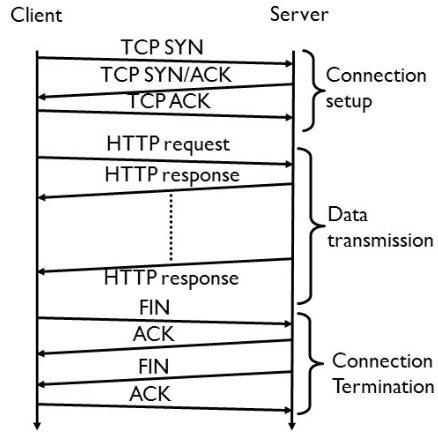
\includegraphics[width=8cm]{./02_Capitulos/02_Cap3/figures/http-flow}
\caption{Fluxo de conexão do HTTP}
\label{fig:3.2.0/http-flow}
\end{figure}

MQTT é um protocolo com cabeçalhos menores, conexão persistente e menos passos para o envio de mensagem, como visto na \ref{fig:3.2.0/mqtt-flow}. Por ser um protocolo feito com o objetivo de reduzir a latência, leva vantagem para a transmissão contínua de dados  em relação ao HTTP.

\begin{figure}[h!]
\centering
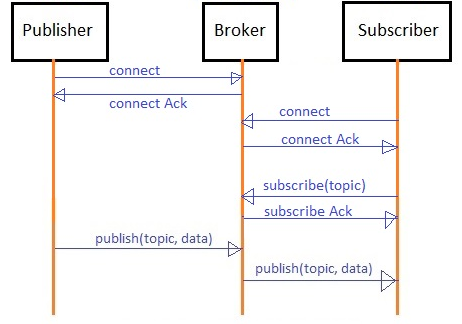
\includegraphics[width=10cm]{./02_Capitulos/02_Cap3/figures/mqtt-flow}
\caption{Fluxo da conexão do MQTT}
\label{fig:3.2.0/mqtt-flow}
\end{figure}

Abaixo na \ref{tabela:mqttxhttp} encontra-se o resumo comparativo entre os protocolos MQTT e HTTP:

\begin{table}[h!]
\caption{Comparativo MQTT X HTTP}
\resizebox{\textwidth}{!}{%
\begin{tabular}{|l|l|l|}
\hline
\textbf{Característica-Protocolo}     & \textbf{MQTT}                           & \textbf{HTTP}         \\ \hline
\textbf{Arquitetura}                  & Publish/Subscribe                       & Request/Response      \\ \hline
\textbf{Complexidade}                 & simples                                 & complexa              \\ \hline
\textbf{Segurança}                    & TSL/SSL                                 & TSL/SSL               \\ \hline
\textbf{Camada de Transporte}         & TCP                                     & TCP ou UDP            \\ \hline
\textbf{Tamanho/Formato de Mensagens} & curtas, binário com cabeçalho de 2Bytes & Grande, Formato ASCII \\ \hline
\textbf{Porta Padrão}                 & 1883                                    & 80 ou 8080            \\ \hline
\textbf{Distribuição de dados}        & 1 um para 0/1/N                         & um para um            \\ \hline
\end{tabular}%
}
\label{tabela:mqttxhttp}
\end{table}


\subsection{Publishers e Subscribers}
\label{subsection:publishers_subscribers}

Para enviar e receber dados de uma forma a atender os requisitos da seção \ref{section:interface_iot}, foi utilizado um padrão de comunicação recorrente em aplicações contemporâneas, o padrão Publish/Subscriber \cite{amazon:pub-sub}.

O padrão Publish/Subscribe permite que as mensagens sejam transmitidas assíncronas e para vários dispositivos simultaneamente. Para transmitir uma mensagem, um cliente pode simplesmente enviar uma mensagem para um determinado tópico. Todos os componentes que se inscreverem no tópico receberão todas as mensagens transmitidas, a menos que uma política de filtragem de mensagens seja definida pelo assinante do tópico.

\begin{figure}[h!]
\centering
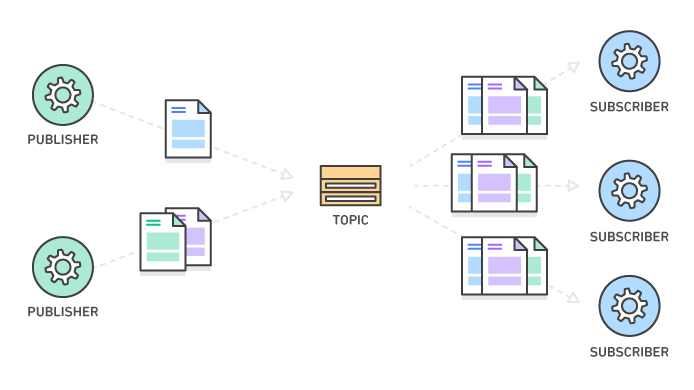
\includegraphics[width=12cm]{./02_Capitulos/02_Cap3/figures/aws_pub_sub}
\caption{O padrão Publish/Subscribe. Retirado de \cite{amazon:pub-sub}}
\label{fig:3.2.0/aws_pub_sub}
\end{figure}

Qualquer mensagem publicada em um tópico é imediatamente recebida por todos os assinantes deste tópico. Com isso, foram criados duas funções possíveis para cada dispositivo dentro deste padrão, os Publishers, quem enviarão as mensagens de dados e os Subscribers, quem receberão. Sua comunicação é ilustrada na \ref{fig:3.2.0/pub_sub}.

\subsection{Broker}
\label{subsection:broker}

O Broker é o servidor do padrão Publish/Subscribe, ele efetivamente executa as ordens de publicação (publish) feita por algum cliente para os tópicos que outros clientes estão inscritos (subscribed), possui todas as listas de tópicos, é orientado a conexão e não persiste informações dos clientes, ou seja, em caso de queda de conexão, estes devem se inscrever novamente nos tópicos.  A arquitetura Broker não é exclusividade do MQTT, outros protocolos utilizam esse tipo de implementação em servidores em arquiteturas semelhantes de envio de mensagem, como os Hubs desenvolvidos pela Microsoft na biblioteca SignalR \cite{signalr}.

\begin{figure}[h]
\centering
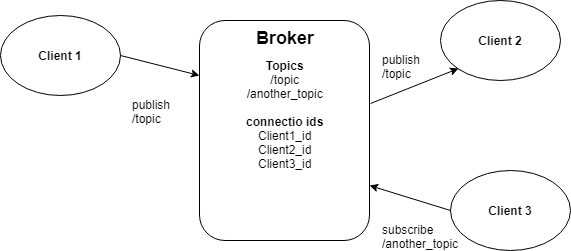
\includegraphics[width=12cm]{./02_Capitulos/02_Cap3/figures/broker_pub_sub}
\caption{Exemplo de gerênciamento de um broker}
\label{fig:3.2.0/broker_pub_sub}
\end{figure}

Na figura \ref{fig:3.2.0/broker_pub_sub}, o Broker armazena os tópicos e os Ids de conexão dos clientes, 2 estava inscrito para ouvir as mensagens do tópico \textit{topic}, enquanto 3 enviava uma ordem de inscrição em \textit{another\_topic} e o cliente 1 envia ordem de publicação para \textit{topic}.


\subsection{Tipos de MQTT}
\label{subsection:tipos_mqtt}

%% Tipos de MQTT 
Com a evolução e o uso do protocolo, foram necessárias atualizações que contemplam funcionalidades que atendem  requisitos essenciais para aplicações da indústria. Dentre esses requisitos, tem-se atender dispositivos que não usam a pilha TCP/IP e medidas de segurança da informação nas mensagens enviadas. 

Existe uma gama de dispositivos que utilizam protocolos específicos, não construídos sobre o TCP/I, a exemplo do ZigBee \cite{zigbee}. Para isso foi criada uma versão do MQTT para atender estes tipos de protocolos, substituindo a base TCP/IP por outros protocolos destas camadas, mantendo a camada de aplicação e o padrão Publish/Subscribe.

Para resolver questões de segurança, foi criada uma variação do MQTT que adiciona camadas deste quesito ao protocolo de aplicação. Assim como o HTTPS o protocolo MQTTS é construído em cima do protocolo SSL/TLS \cite{ssl}, camada de segurança construídas sobre TCP/IP. Esta camada envolve o processo de encriptação dos cabeçalhos da aplicação e autenticação por certificados. Para poder criar uma conexão é requisitado um certificado SSL, durante o processo de solicitação do certificado SSL, a Autoridade de Certificação validará seus detalhes, permitindo a passagem de dados encriptados.

\section{Persistência de dados}
\label{section:persistencia}

%% Bancos de dados
Os dados adquiridos pela plataforma e suas camadas, são armazenados em memórias e enviados. Memórias voláteis que podem facilmente perder dados com quedas de energia ou por conta da reutilização do espaço da memória, para garantir que os dados não sejam perdidos, é necessário que o sistema possua persistência, uma forma de memória não-volátil que armazene os dados sem energia.

Essa persistência é implementada com Banco de Dados, que são estruturas que organizam o armazenamento de dados persistentes em arquivos. Um Banco de dados é  basicamente uma aplicação, um serviço do sistema que recebe requisições de rede e escreve ou lê dados em um arquivo. Existem inúmeras formas de implementação e protocolos de comunicação para Bancos de Dados.

Um banco é composto por duas ferramentas, o Motor e o Arquivo de dados. O motor é quem realiza as ações sobre o arquivo,ou seja, é o sistema de gerenciamento. Recebe as requisições e aplica algoritmos de escrita de dados eficientes no arquivo para armazenar os dados em uma estrutura definida pelo próprio motor, baseado em algoritmos de estrutura de dados. Um Banco de dados pode possuir vários motores, cada um com um algoritmo de distinta eficiência em termos de tempo de escrita e/ou leitura de acordo com o dado recebido.

\begin{figure}[h!]
\centering
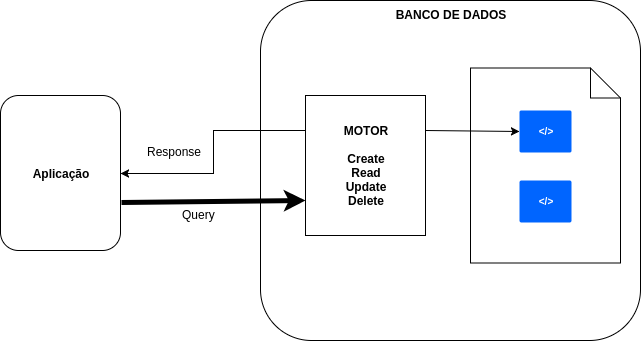
\includegraphics[width=12cm]{./02_Capitulos/02_Cap3/figures/Database_Arch}
\caption{A arquitetura de um banco de dados}
\label{fig:3.3.5/database_arch}
\end{figure}

O arquivo é o documento onde os dados são armazenados. A forma de armazenamento de dados define a eficiência do motor em buscar e escrever dados, então e necessário a escolha adequada do algoritmo para uma maior eficiência da leitura do arquivo, como em \ref{fig:3.3.5/database_arch}, a aplicação envia uma solicitação de criação, leitura, atualização ou remoção (CRUD - Create, Read, Update, Delete) e o motor escreve (ou lê) do arquivo.


 
\section{Bancos para Aplicações IoT}
\label{section:bancos_IoT}


Como pode ser observado em \cite{Damodaran}, uma aplicação eficiente de Bancos de Dados em IoT está ligada ao tempo de inserção de dados no banco, ou seja,  o tempo total em que a aplicação leva para enviar e inserir o dado no documento e de fato armazenar. Podem ser feitas várias inserções de pequenos pacotes de dados, dependendo do tamanho da mensagem. Esta característica está ligada ao motor do banco, que determina como o dado será armazenado, e quanto tempo ele leva para escrever o dado no documento. A maioria dos dados são armazenados em estruturas de árvore B+ \cite{b-tree}, porém pode-se observar em \cite{Damodaran} que a estrutura de árvore LSM  \cite{O'Neal-Gawlick-Cheng} possui maior eficiência na escrita.


\begin{figure}[h!]
\centering
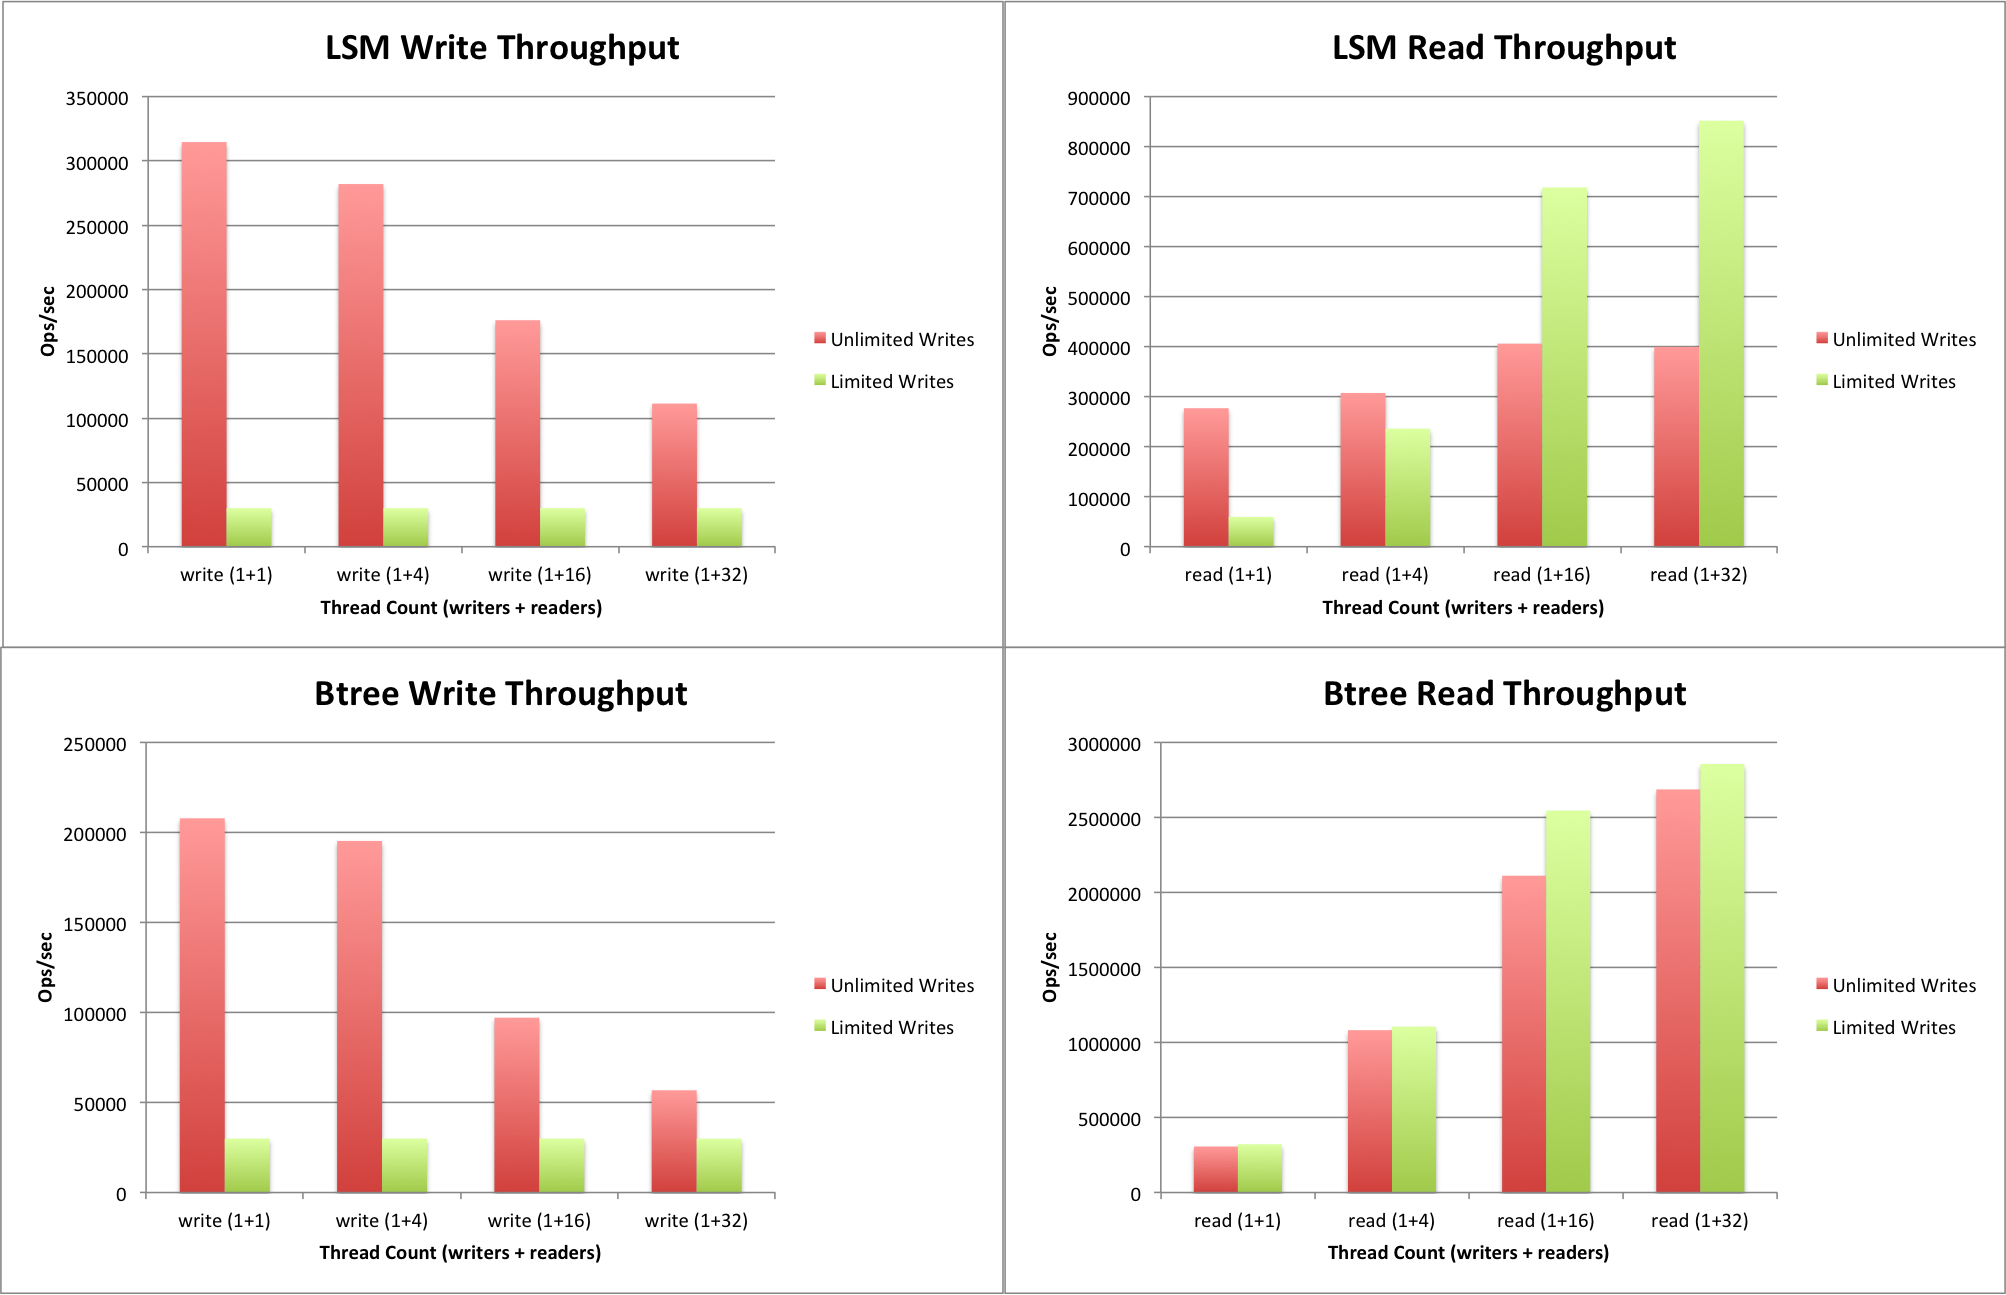
\includegraphics[width=14cm]{./02_Capitulos/02_Cap3/figures/LSM_btree}
\caption{Comparação de Escrita e Leitura entre LSM e B+, retirado de \cite{btrees-vs-lsmtrees}}
\label{fig:3.3.5/b-lsm}
\end{figure}

Comparando as duas estruturas, como mostrado em \ref{fig:3.3.5/b-lsm}, percebe-se que a estrutura LSM sustenta até 2x mais inserções da estrutura B+, hoje os Bancos de Dados modernos utilizam desta vantagem. Aplicações modernas coletam dados constantemente, então a eficiência da operação de escrita feita por um motor de um banco torna-se extremamente relevante, a estrutura LSM leva vantagem neste quesito.

Existem várias abstrações de Bancos de dados. Em \cite{Rautmare-Bhalerao} compara-se e conclui-se que o banco MongoDB, um banco NoSQL possui um tempo de resposta de inserção menor que o MySQL (bancos relacionais), porém o último é mais estável. De fato, bancos NoSQL (bancos não-relacionais) são, em geral, mais leves e possuem uma flexibilidade maior para lidar e estruturar dados, o que fazem estes tipos de Banco mais favoráveis a aplicações de IoT, porém outras estruturas como um banco divido em séries de tempo \cite{timeseries} , onde a indexação dos dados é feita pelo tempo de quando a amostra foi coletada (isso será debatido em \ref{section:timestamp}), mostram-se eficientes com bancos relacionais ou não.

Outros aspectos podem contribuir para a eficiência de persistência de dados. Criar bancos locais diminuem a latência e a necessecidade de conexão, aumentando a capacidade de inserção de dados, além de ser uma forma de backup de dados. Um banco local, geralmente fica em uma plataforma como em \cite{Paethong-Sato-Namiki}, são bancos leves em aplicações de baixo consumo, devido a capacidade de processamento limitada. Seu papel é geralmente para armazenar os dados quando não há conexão, e quando esta é restabelecida os dados são enviados para um banco remoto com mais capacidade de processamento e aplicações. %% Falar sobre bancos locais.

Dentre os bancos estudados, alguns se destacam como o Cassandra, usado pela Netflix para coletar dados sobre o comportamento do usuário na plataforma ou o InfluxDB, um banco em série de temo, feito para aplicações em tempo real. Mas para esse projeto, foi utilizado o MongoDB \cite{mongodb}, um banco NoSQL, leve e de fácil integração com as plataformas utilizadas e que possui implementações de motores que priorizam a eficiência na escrita de dados, como a LSM tree.




